
%(BEGIN_QUESTION)
% Copyright 2010, Tony R. Kuphaldt, released under the Creative Commons Attribution License (v 1.0)
% This means you may do almost anything with this work of mine, so long as you give me proper credit

A common ``accessory'' device for a variable-frequency drive (VFD) is a {\it line reactor}, which is nothing more than a large inductor connected in series with each of the motor drive's power line conductors.  The purpose of a line reactor is to act as a low-pass filter, allowing 60 Hz power to the VFD but blocking harmonic frequencies generated by the VFD from ``corrupting'' the AC power supply system.

$$\includegraphics[width=15.5cm]{i03242x01.eps}$$

Suppose each winding of a line reactor for a 10 horsepower VFD has 0.119 $\Omega$ of resistance and 1.5 mH of inductance.  Calculate the amount of {\it impedance} offered by each winding to the following harmonics:

% No blank lines allowed between lines of an \halign structure!
% I use comments (%) instead, so that TeX doesn't choke.

$$\vbox{\offinterlineskip
\halign{\strut
\vrule \quad\hfil # \ \hfil & 
\vrule \quad\hfil # \ \hfil \vrule \cr
\noalign{\hrule}
%
% First row
Frequency ($f$) & Impedance ($Z$) \cr
%
\noalign{\hrule}
%
% Another row
60 Hz (1st harmonic) &  \cr
%
\noalign{\hrule}
%
% Another row
180 Hz (3rd harmonic) &  \cr
%
\noalign{\hrule}
%
% Another row
300 Hz (5th harmonic) &  \cr
%
\noalign{\hrule}
%
% Another row
420 Hz (7th harmonic) &  \cr
%
\noalign{\hrule}
%
% Another row
540 Hz (9th harmonic) &  \cr
%
\noalign{\hrule}
} % End of \halign 
}$$ % End of \vbox

Hint: you may consider each reactor coil to be a series-connected inductor and resistor, together producing a certain amount of impedance for each frequency.

\vfil

\underbar{file i03242}
\eject
%(END_QUESTION)





%(BEGIN_ANSWER)

This is a graded question -- no answers or hints given!
 
%(END_ANSWER)





%(BEGIN_NOTES)

Recall that the reactance of an inductor may be calculated by the following formula:

$$X_L = 2 \pi f L$$

Recall as well that the total impedance of a series reactance-resistance network is predicted by the following formula:

$$\sqrt{R^2 + X^2}$$

The rest is simply calculating impedance for each of the harmonic frequencies, one at a time:

% No blank lines allowed between lines of an \halign structure!
% I use comments (%) instead, so that TeX doesn't choke.

$$\vbox{\offinterlineskip
\halign{\strut
\vrule \quad\hfil # \ \hfil & 
\vrule \quad\hfil # \ \hfil \vrule \cr
\noalign{\hrule}
%
% First row
Frequency ($f$) & Impedance ($Z$) \cr
%
\noalign{\hrule}
%
% Another row
60 Hz (1st harmonic) & 0.578 $\Omega$ \cr
%
\noalign{\hrule}
%
% Another row
180 Hz (3rd harmonic) & 1.701 $\Omega$ \cr
%
\noalign{\hrule}
%
% Another row
300 Hz (5th harmonic) & 2.830 $\Omega$ \cr
%
\noalign{\hrule}
%
% Another row
420 Hz (7th harmonic) & 3.960 $\Omega$ \cr
%
\noalign{\hrule}
%
% Another row
540 Hz (9th harmonic) & 5.091 $\Omega$ \cr
%
\noalign{\hrule}
} % End of \halign 
}$$ % End of \vbox

As you can see, the line reactors present a much higher amount of impedance to harmonic currents than to the fundamental (60 Hz) current, and so tend to filter those harmonic currents from reaching the 3-phase 480 VAC power source where they might cause problems with other circuit components.

%INDEX% Electronics review: inductive reactance and harmonic frequencies

%(END_NOTES)


